\chapter{Dữ liệu và phương pháp nghiên cứu}
\label{ch:phuong-phap}

Chương này trình bày kiến trúc hệ thống, quy trình xử lý dữ liệu và thiết kế các mô hình học máy trong khung thực nghiệm DepSev-ML. Phương pháp luận được xây dựng dựa trên ba nguyên tắc: module hóa, kiểm soát chặt chẽ quy trình tiền xử lý nhằm loại bỏ rò rỉ dữ liệu (Zero Data Leakage), và thử nghiệm đa dạng các trường phái mô hình hóa từ phân loại phẳng, phân cấp đến thứ bậc.

\section{Tổng quan quy trình nghiên cứu DepSev-ML}
\label{sec:kien-truc-tong-the}

Quy trình thực nghiệm DepSev-ML được tổ chức thành 7 bước tuần tự như mô tả trong Hình \ref{fig:overall-architecture}.

\begin{figure}[htbp]{Sơ đồ quy trình nghiên cứu thực nghiệm 7 bước của khung DepSev-ML.}
\centering
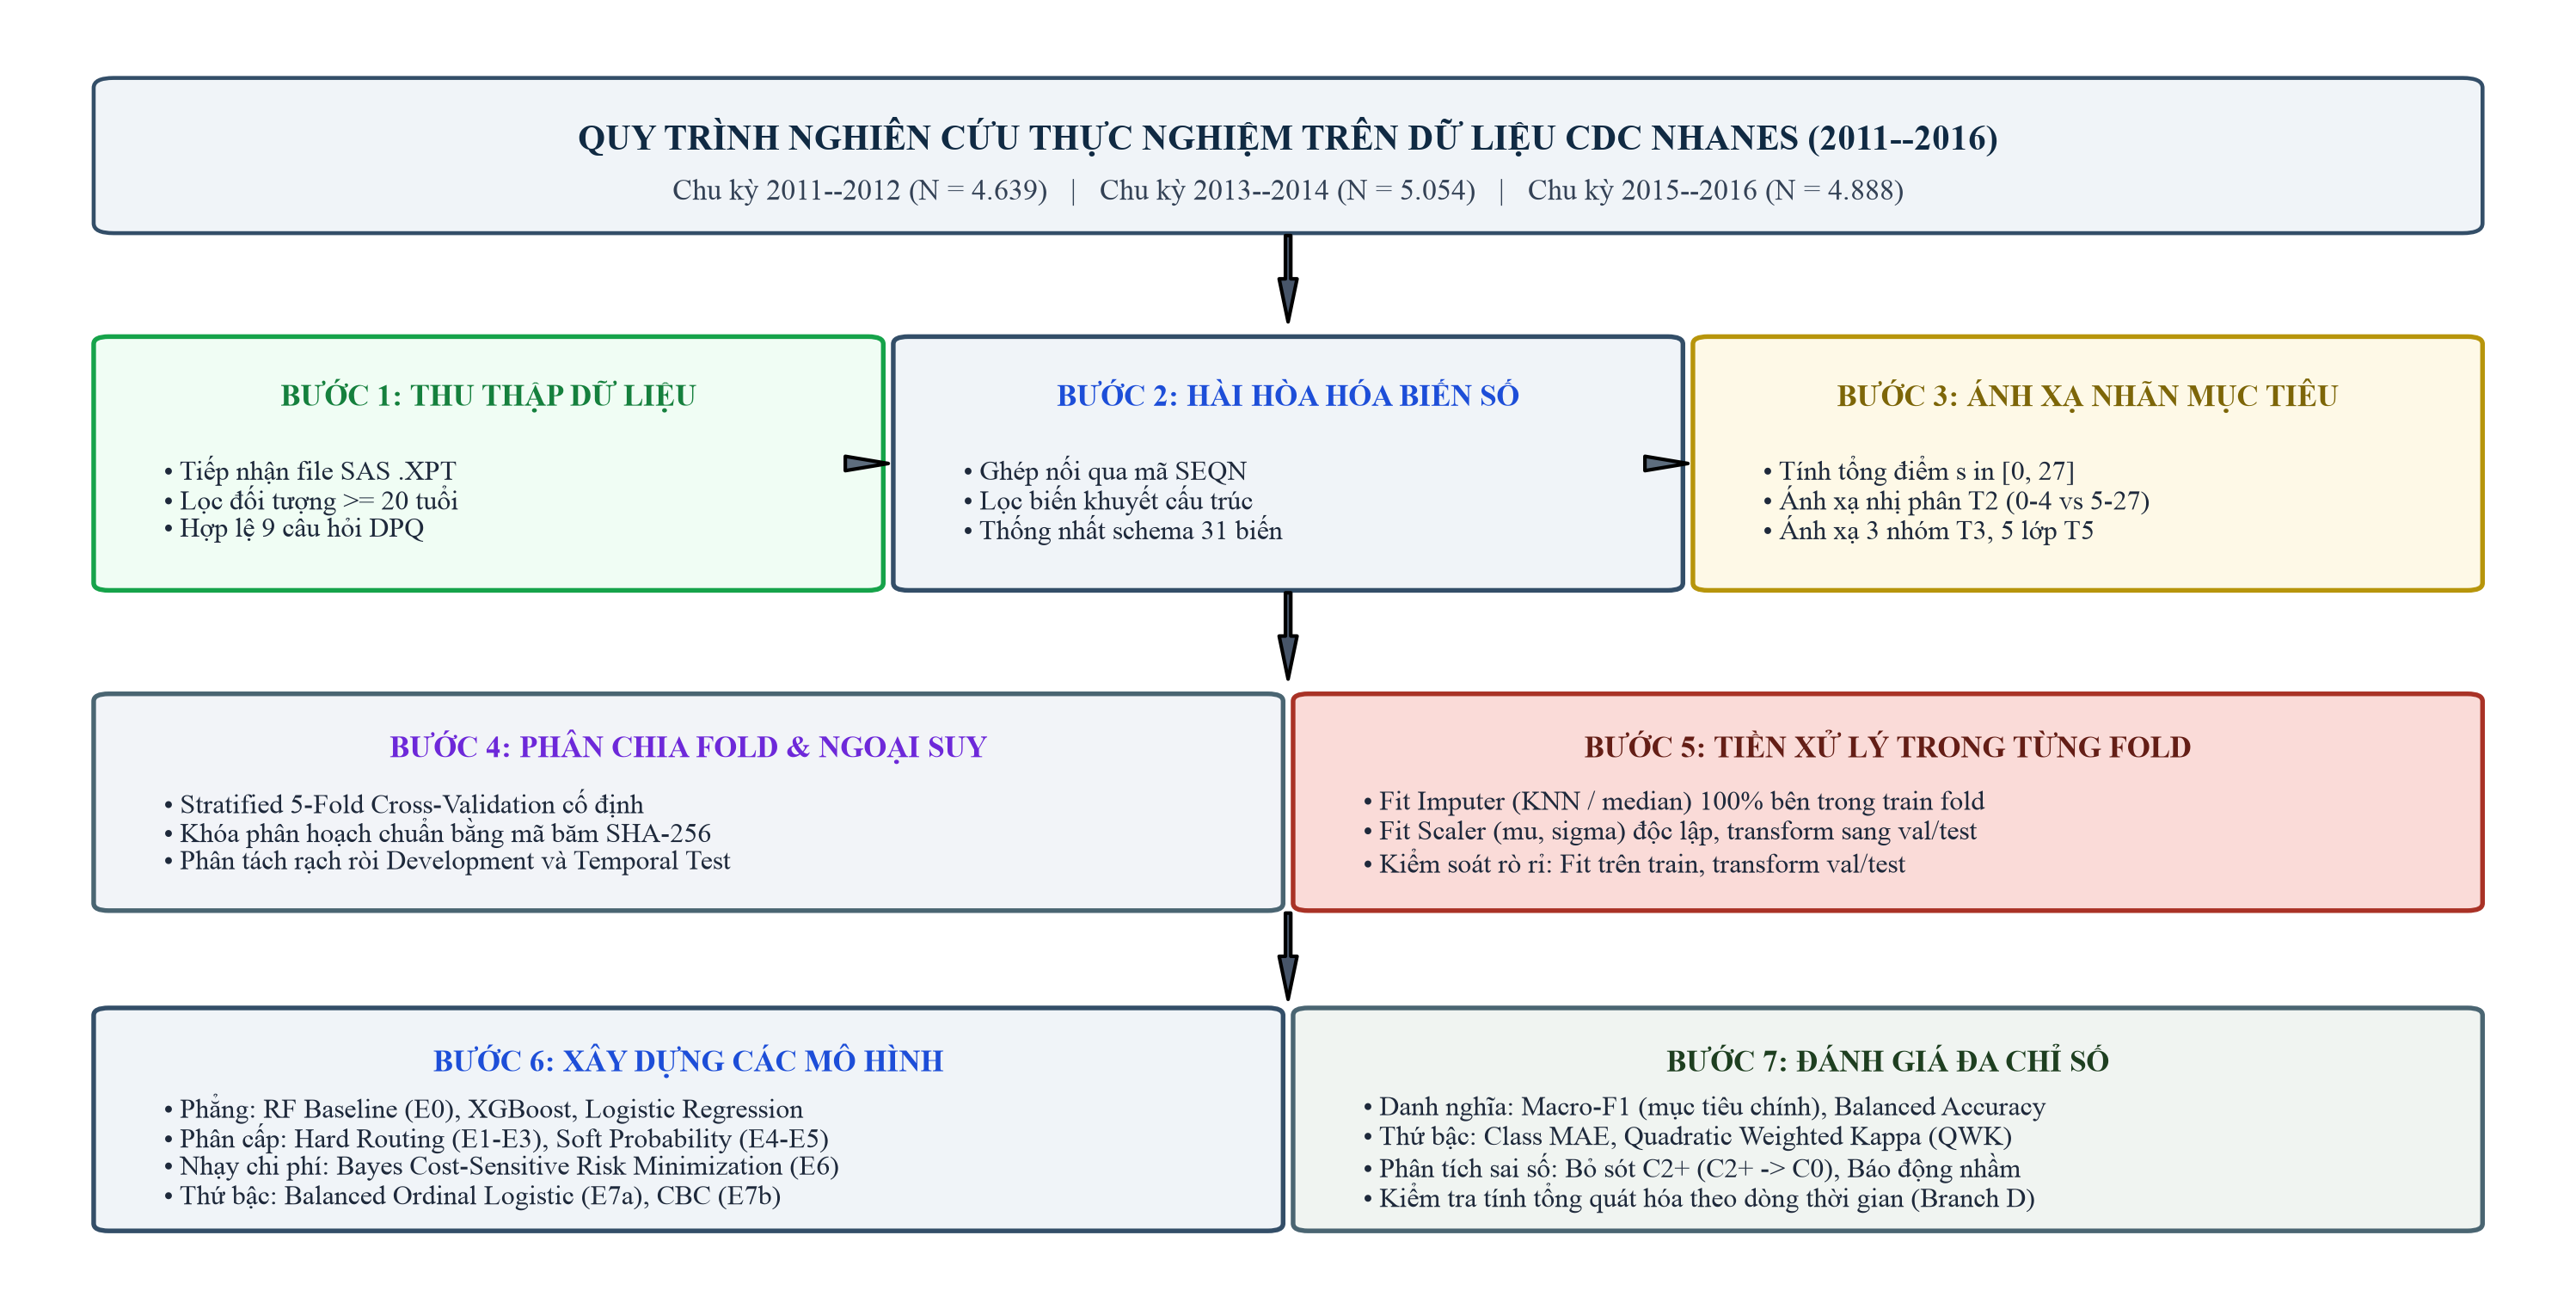
\includegraphics[width=0.92\textwidth]{figures/depsev_overall_architecture.png}
\label{fig:overall-architecture}
\end{figure}

Các bước thực hiện các chức năng cụ thể:
\begin{enumerate}
    \item \textit{Bước 1 -- Tiếp nhận và lọc đối tượng (Cohort Intake):} Tiếp nhận các tệp dữ liệu gốc định dạng SAS Transport (.XPT) từ CDC/NCHS, lọc đối tượng người trưởng thành ($\text{RIDAGEYR} \ge 20$) có đủ 9 mục khảo sát PHQ-9 hợp lệ.
    \item \textit{Bước 2 -- Hài hòa hóa và trích xuất đặc trưng:} Ghép nối các bảng khảo sát qua mã định danh SEQN; chuẩn hóa tên biến và loại bỏ các biến có tỷ lệ khuyết thiếu quá cao hoặc thay đổi định nghĩa giữa các chu kỳ.
    \item \textit{Bước 3 -- Thiết lập không gian nhãn mục tiêu:} Ánh xạ tổng điểm PHQ-9 thành các không gian nhãn rời rạc ($T_2, T_3, T_4, T_5$) phục vụ phân tích đa độ phân giải.
    \item \textit{Bước 4 -- Phân hoạch dữ liệu có kiểm soát:} Quản lý các phân hoạch dữ liệu cố định (Stratified 5-Fold CV) bằng mã băm kiểm tra nhằm bảo đảm tính tái lập thực nghiệm tuyệt đối.
    \item \textit{Bước 5 -- Tiền xử lý dữ liệu in-fold:} Thực hiện điền khuyết (median/mode) và chuẩn hóa độc lập hoàn toàn bên trong từng fold huấn luyện.
    \item \textit{Bước 6 -- Triển khai các hướng mô hình hóa ($E_0 \to E_7$):} Huấn luyện mô hình phân loại phẳng cơ sở, các cấu hình phân cấp định tuyến cứng, phân cấp định tuyến mềm kết hợp chi phí Bayes và mô hình phân loại thứ bậc.
    \item \textit{Bước 7 -- Đánh giá hiệu năng đa chiều:} Đo lường qua hệ thống chỉ số danh nghĩa (Macro-F1, Balanced Accuracy), chỉ số thứ bậc (Class MAE, QWK) và tiêu chí an toàn y tế (số ca nặng bị bỏ sót $C_2^+ \to C_0$).
\end{enumerate}

\section{Bộ dữ liệu NHANES và quy trình tiền xử lý in-fold}
\label{sec:du-lieu-nghien-cuu}

\subsection{Tập dữ liệu phát triển Legacy (NHANES 2013--2014)}
\label{subsec:legacy-cohort}

Tập dữ liệu phát triển chính được xây dựng từ chu kỳ NHANES 2013--2014, gồm $N = 4.045$ đối tượng trưởng thành có đầy đủ dữ liệu khảo sát và cận lâm sàng:
\begin{itemize}
    \item Lớp $C_0$ (Tối thiểu, 0--4 điểm): $3.080$ mẫu (chiếm 76.14\%).
    \item Lớp $C_1$ (Nhẹ, 5--9 điểm): $667$ mẫu (chiếm 16.49\%).
    \item Lớp $C_2^+$ (Nặng quy ước, $\ge 10$ điểm): $298$ mẫu (chiếm 7.37\%), gồm 189 ca vừa ($C_2$), 65 ca nặng vừa ($C_3$) và 44 ca nặng ($C_4$).
\end{itemize}

\subsection{Quy trình tiền xử lý in-fold và kiểm soát rò rỉ dữ liệu}
\label{subsec:infold-preprocessing}

Để bảo đảm tính khách quan khoa học, toàn bộ các bước tiền xử lý đều được thực hiện theo nguyên tắc in-fold nghiêm ngặt (Hình \ref{fig:infold-pipeline}).

\begin{figure}[htbp]{Quy trình tiền xử lý in-fold và phân tách kiểm định chéo bảo đảm Zero Data Leakage.}
\centering
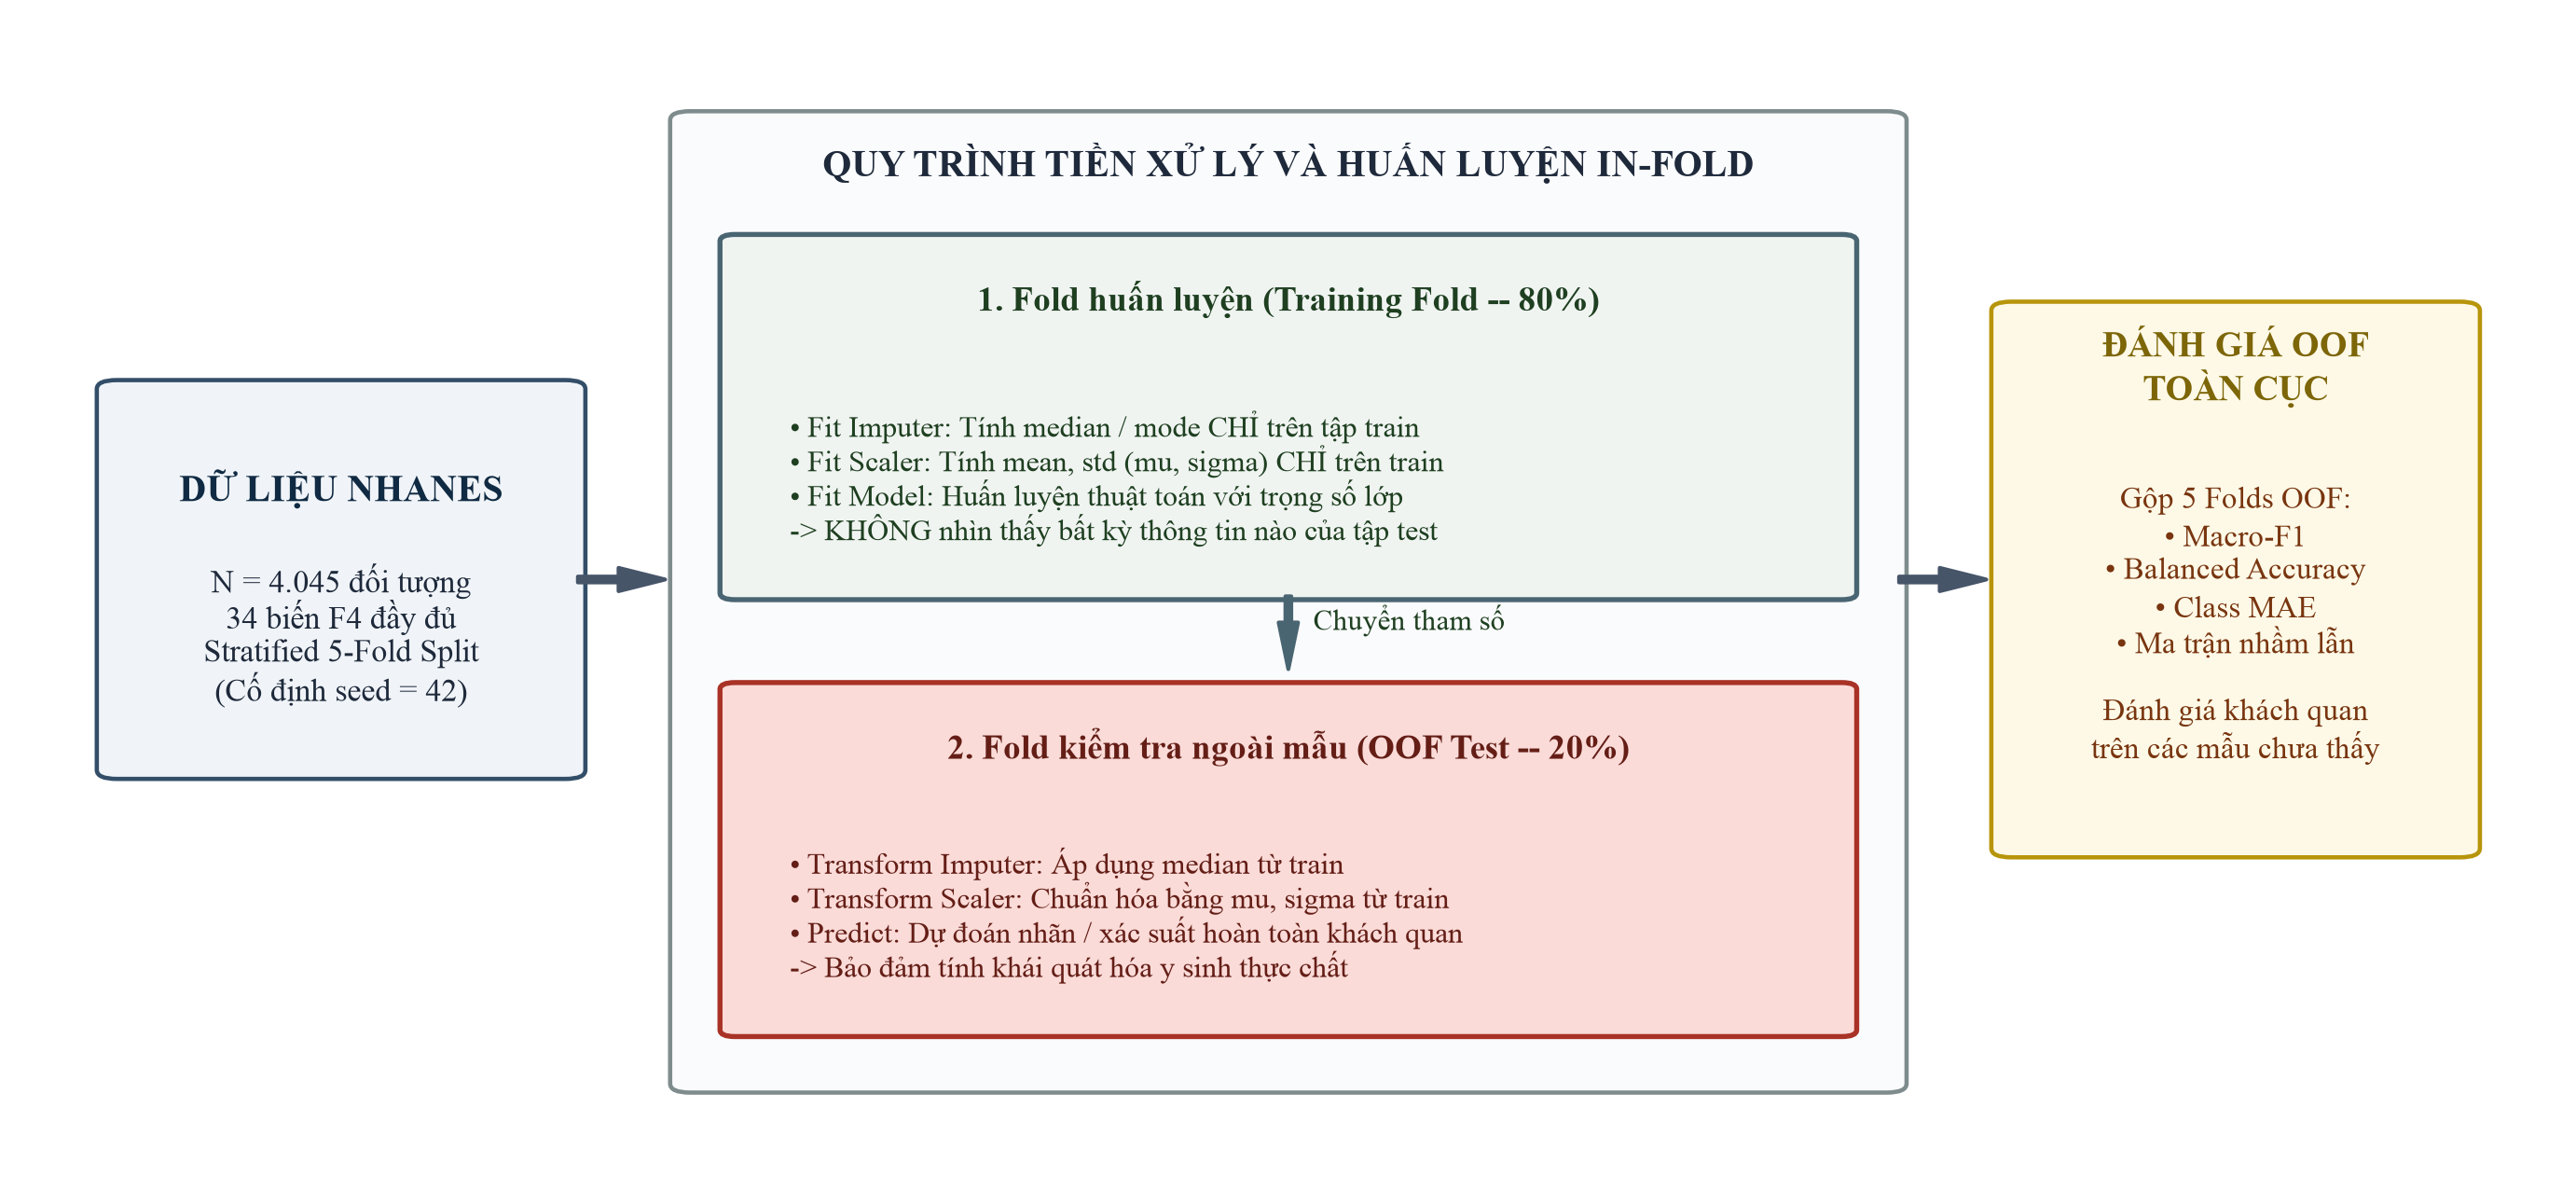
\includegraphics[width=0.92\textwidth]{figures/fig3_infold_cv_pipeline.png}
\label{fig:infold-pipeline}
\end{figure}

Các tham số thống kê (như giá trị trung vị dùng để điền khuyết hay giá trị trung bình và độ lệch chuẩn dùng để chuẩn hóa thang đo) chỉ được tính toán duy nhất trên tập huấn luyện của fold hiện tại. Tập kiểm thử của fold đó hoàn toàn bị cô lập và chỉ sử dụng các tham số đã đóng băng từ tập huấn luyện để chuyển đổi. Cơ chế này loại bỏ hoàn toàn nguy cơ rò rỉ phân phối từ tập kiểm tra vào tập huấn luyện.

\subsection{Bản chất khoa học của tập đặc trưng rút gọn $F_{4\_\text{common31}}$}
\label{subsec:common31-definition}

Để phục vụ kiểm định ngoại suy sang chu kỳ độc lập NHANES 2015--2016, tập đặc trưng chuẩn $F_4$ (gồm 34 biến) được điều chỉnh thành tập rút gọn $F_{4\_\text{common31}}$ (gồm 31 biến):
\begin{itemize}
    \item \textit{Làm rõ về biến Triglycerides (LBXTR):} Biến Triglycerides chưa từng nằm trong tập 34 đặc trưng đóng băng của $F_4$. Do nằm trong nhóm xét nghiệm nhịn ăn buổi sáng với tỷ lệ khuyết thiếu $>50\%$, biến này đã bị loại bỏ ngay từ khâu lọc intake ban đầu khi xây dựng cohort.
    \item \textit{3 biến thực sự bị loại bỏ từ $F_4$ xuống $F_{4\_\text{common31}}$:} Qua kiểm tra mã nguồn tại \textnormal{src/common31\_features.py}, 3 đặc trưng bị thay đổi định nghĩa câu hỏi hoặc không xuất hiện trong chu kỳ 2015--2016 gồm: (1) \textit{SLD010H} (số giờ ngủ mỗi đêm); (2) \textit{PAQ605} (hoạt động thể lực cường độ mạnh trong công việc); và (3) \textit{PAD680} (thời gian ngồi tĩnh tại mỗi ngày). Ngoài ra, biến lượng rượu tiêu thụ được tiến hành top-coding ở ngưỡng 15 ly/ngày để tương thích phân phối.
\end{itemize}

\section{Xây dựng không gian đặc trưng lũy tiến ($F_1 \to F_4$)}
\label{sec:khong-gian-dac-trung}

Để đánh giá định lượng đóng góp của từng nhóm yếu tố, nghiên cứu thiết kế 4 không gian đặc trưng tích lũy tăng dần:
\begin{itemize}
    \item \textit{Không gian $F_1$ (Nhân khẩu học -- 4 đặc trưng):} Tuổi (RIDAGEYR), giới tính (RIAGENDR), chủng tộc (RIDRETH3) và tỷ lệ thu nhập trên ngưỡng nghèo (INDFMPIR).
    \item \textit{Không gian $F_2$ ($F_1$ + Lối sống và Tiền sử -- 13 đặc trưng):} Bổ sung tình trạng hút thuốc, uống rượu, hoạt động thể chất, giấc ngủ và tiền sử các bệnh mạn tính (tiểu đường, tim mạch, đột quỵ).
    \item \textit{Không gian $F_3$ ($F_2$ + Đo lường thể chất -- 19 đặc trưng):} Bổ sung chỉ số khối cơ thể (BMXBMI), chu vi vòng eo (BMXWAIST), nhịp tim và các số đo huyết áp (huyết áp tâm thu SBP, huyết áp tâm trương DBP).
    \item \textit{Không gian $F_4$ ($F_3$ + Sinh hóa máu -- 34 đặc trưng):} Bổ sung 15 chỉ số xét nghiệm cận lâm sàng gồm công thức máu (bạch cầu WBC, hồng cầu RBC, tiểu cầu PLT), chuyển hóa (glucose, HbA1c, albumin) và lipid máu (cholesterol toàn phần, HDL).
\end{itemize}

\section{Thiết kế các kiến trúc mô hình thực nghiệm ($E_0 \to E_7$)}
\label{sec:thiet-ke-mo-hinh}

Trên không gian bài toán 3 nhóm ($T_3$), nghiên cứu triển khai 12 cấu hình mô hình thuộc 4 trường phái khác nhau:

\subsection{Mô hình phân loại phẳng cơ sở ($E_0$)}
Sử dụng Random Forest huấn luyện trực tiếp trên không gian 3 lớp, gán nhãn dự đoán theo xác suất lớn nhất: $\hat{y} = \arg\max_{k \in \{0, 1, 2\}} \bar{P}(C_k \mid \mathbf{x})$.

\subsection{Kiến trúc phân cấp hai giai đoạn định tuyến cứng ($E_1 \to E_3$)}
Sơ đồ hoạt động được thể hiện trong Hình \ref{fig:hard-hierarchical}. Giai đoạn 1 sử dụng Frozen RF để sàng lọc nhị phân: nếu mẫu có xác suất thuộc nhóm không triệu chứng $P(C_0 \mid \mathbf{x}) \ge 0.5$, mẫu được gán ngay nhãn $\hat{y} = C_0$ và kết thúc. Ngược lại, mẫu được chuyển tiếp sang Giai đoạn 2 để phân biệt $C_1$ và $C_2^+$. 

\begin{figure}[htbp]{Kiến trúc phân loại phân cấp định tuyến cứng hai giai đoạn và nút thắt sai số tích lũy.}
\centering
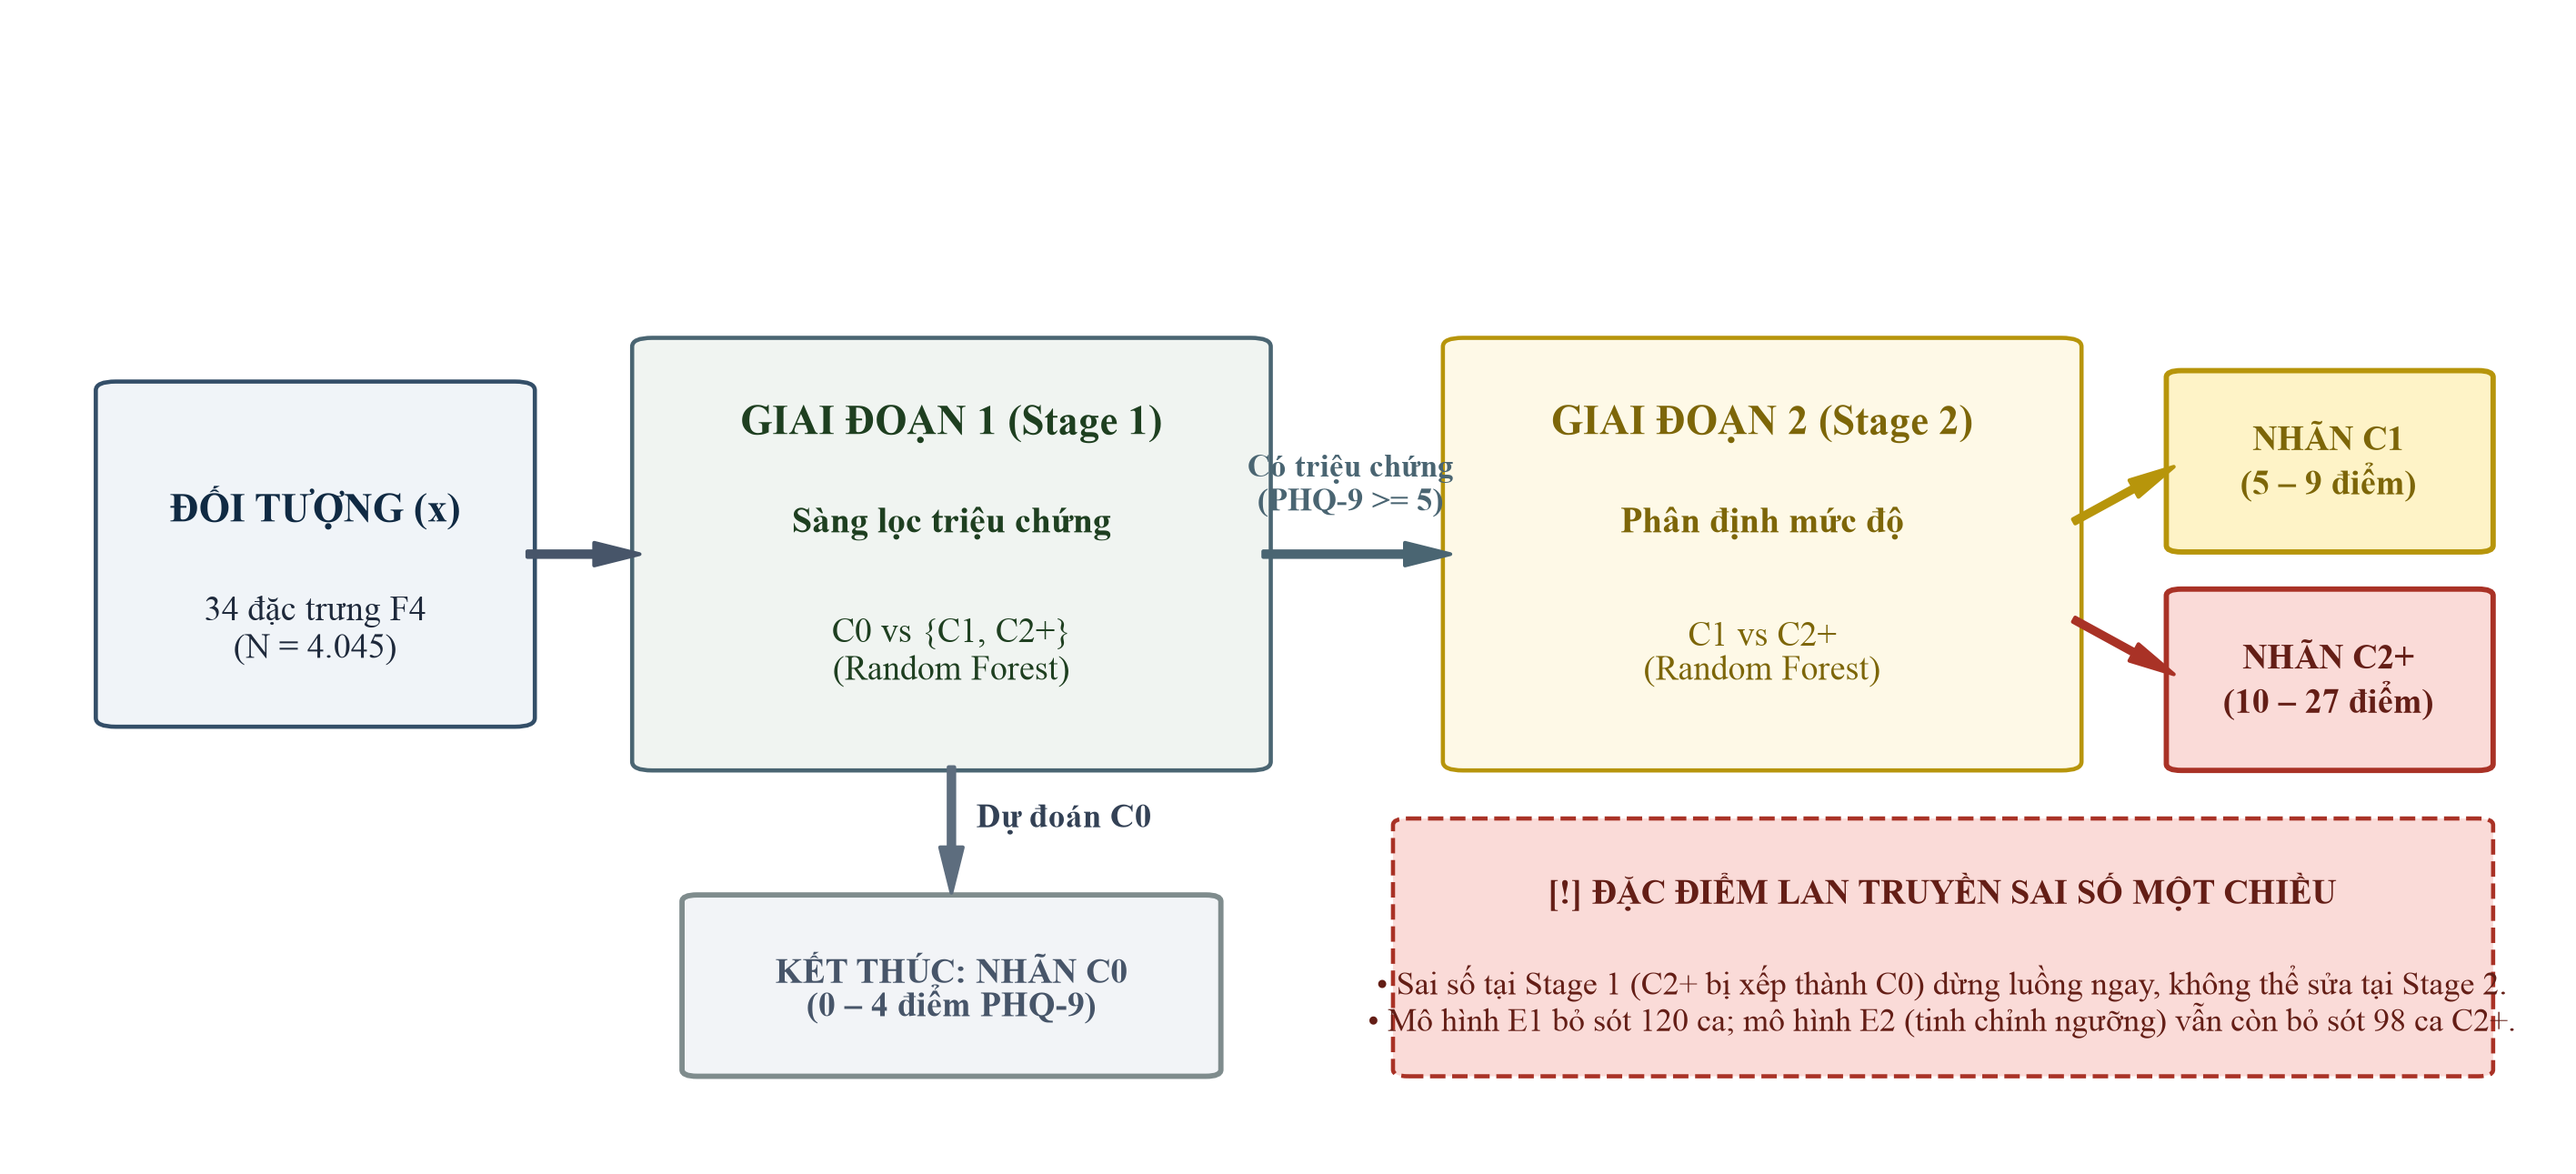
\includegraphics[width=0.92\textwidth]{figures/fig3_4_hard_hierarchical.png}
\label{fig:hard-hierarchical}
\end{figure}

Bốn biến thể thuật toán tại Giai đoạn 2 gồm: Random Forest mặc định ($E_1$), Random Forest tối ưu siêu tham số ($E_2$), XGBoost ($E_{3a}$), và ExtraTrees ($E_{3b}$). Điểm hạn chế cố hữu của cấu trúc cứng là hiện tượng tắc nghẽn sai số: các ca nặng $C_2^+$ bị Giai đoạn 1 gán nhầm thành $C_0$ sẽ hoàn toàn mất cơ hội được xem xét tại Giai đoạn 2.

\subsection{Kiến trúc phân cấp định tuyến mềm và Lý thuyết quyết định Bayes ($E_4 \to E_6$)}
Để khắc phục điểm nghẽn của định tuyến cứng, kiến trúc phân cấp mềm bảo toàn phân phối xác suất liên tục trên toàn bộ quy trình (Hình \ref{fig:soft-hierarchical}).

\begin{figure}[htbp]{Kiến trúc phân loại phân cấp mềm kết hợp Luật quyết định tối ưu chi phí Bayes.}
\centering
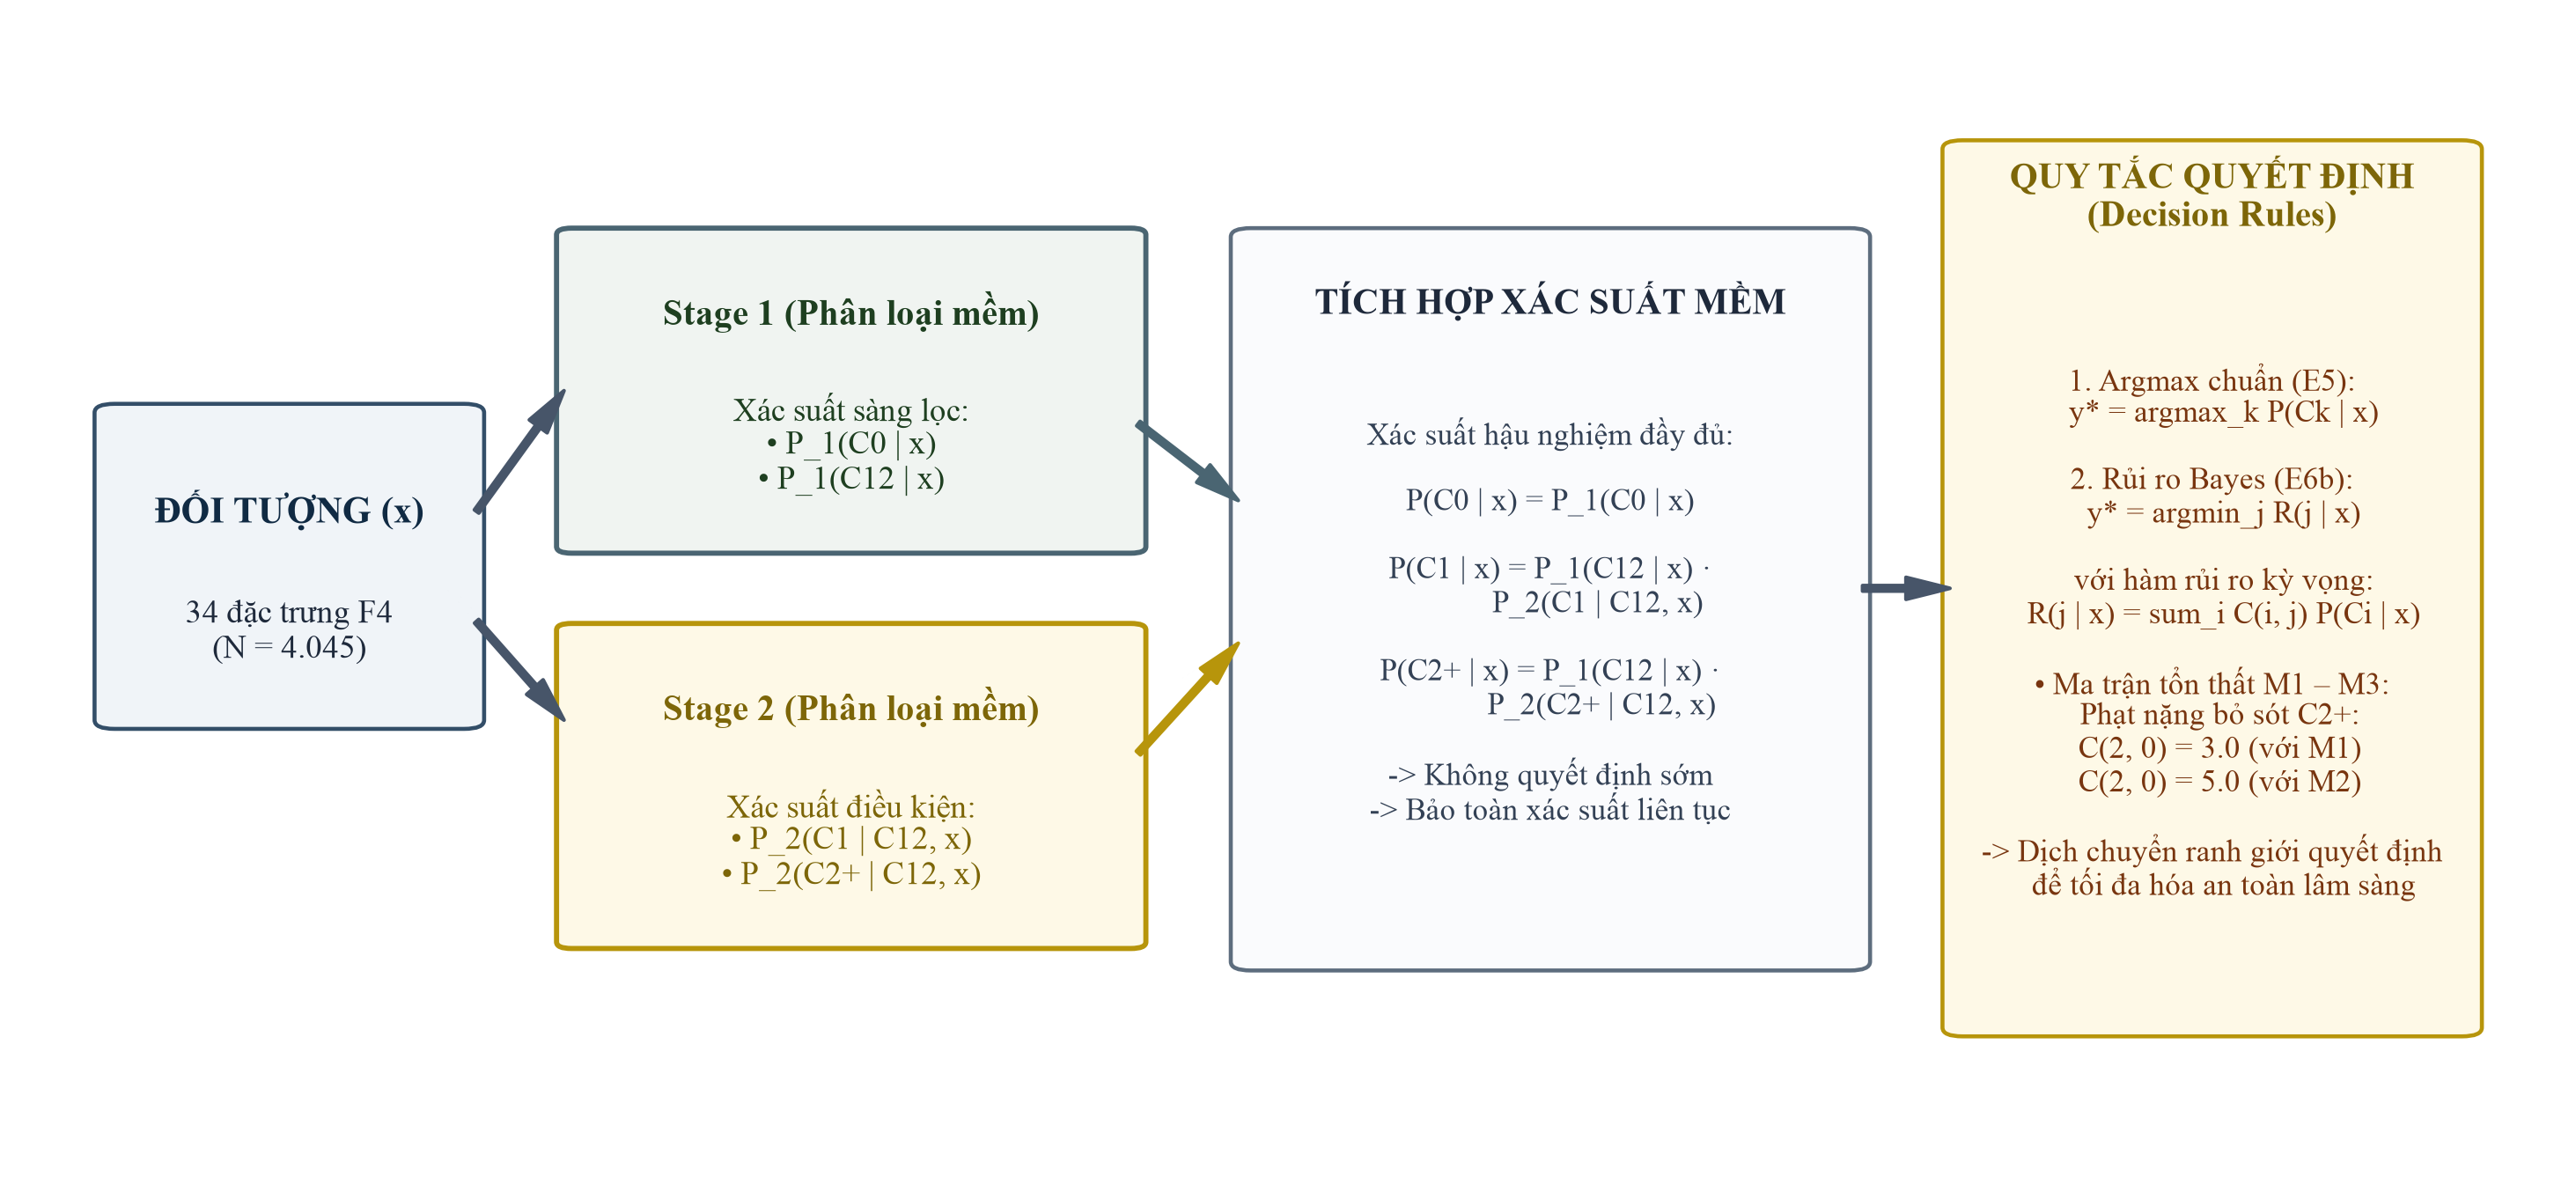
\includegraphics[width=0.92\textwidth]{figures/fig3_5_soft_cost_sensitive.png}
\label{fig:soft-hierarchical}
\end{figure}

Vector xác suất hậu nghiệm toàn thể $\hat{\mathbf{P}} = [\hat{P}_0, \hat{P}_1, \hat{P}_2]^T$ được tính theo công thức xác suất toàn phần:
\begin{align}
    \hat{P}_0(\mathbf{x}) &= P_{\text{stage1}}(C_0 \mid \mathbf{x}) \\
    \hat{P}_1(\mathbf{x}) &= \left[1 - P_{\text{stage1}}(C_0 \mid \mathbf{x})\right] \cdot P_{\text{stage2}}(C_1 \mid \mathbf{x}) \\
    \hat{P}_2(\mathbf{x}) &= \left[1 - P_{\text{stage1}}(C_0 \mid \mathbf{x})\right] \cdot P_{\text{stage2}}(C_2^+ \mid \mathbf{x})
\end{align}

Để tối ưu hóa quyết định dưới sự bất cân xứng rủi ro y tế, quy tắc quyết định Bayes áp dụng ma trận tổn thất $\mathbf{C}$:
\begin{equation}
    \hat{y}^* = \arg\min_{j \in \{0, 1, 2\}} \sum_{i=0}^2 \hat{P}_i(\mathbf{x}) \cdot \mathbf{C}(i, j)
\end{equation}
Nghiên cứu khảo sát 4 ma trận chi phí: $M_0$ (chi phí đều, tương đương luật Argmax $E_5$), $M_1$ (phạt ca bỏ sót $C_2^+ \to C_0$ gấp 10 lần, mô hình $E_{6b}$), $M_2$ (phạt gấp 20 lần), và $M_3$ (ma trận chi phí chuẩn hóa tuyến tính).

\subsection{Mô hình phân loại thứ bậc ($E_7$)}
Khai thác trật tự tự nhiên $C_0 < C_1 < C_2^+$ thông qua hai phương pháp:
\begin{itemize}
    \item $E_{7a}$ (Balanced Ordinal Logistic Regression): sử dụng hàm liên kết logit tích lũy với giả định tỷ lệ chênh tỷ lệ thuận, kết hợp cân bằng trọng số nghịch đảo tần số lớp.
    \item $E_{7b}$ (Cumulative Binary Classification): huấn luyện hai bộ phân loại nhị phân độc lập dự đoán $P(Y \ge 1)$ và $P(Y \ge 2)$, thử nghiệm với bộ phân loại Logistic Regression ($E_{7b}\text{-LR}$) và Random Forest ($E_{7b}\text{-RF}$).
\end{itemize}

\section{Thiết kế giao thức kiểm thử thực nghiệm}
\label{sec:giao-thuc-kiem-thu}

\subsection{Quy trình kiểm định chéo lồng nhau (Nested 5-Fold Stratified CV)}
Để đánh giá không thiên lệch và lựa chọn mô hình cơ sở trên bài toán $T_5$, nghiên cứu áp dụng quy trình kiểm định chéo lồng nhau 5x3:
\begin{itemize}
    \item \textit{Vòng ngoài (Outer Loop):} Phân chia tập dữ liệu thành 5 fold phân tầng. Mỗi lượt giữ lại 1 fold làm tập kiểm tra độc lập để tính toán chỉ số hiệu năng OOF (Out-Of-Fold).
    \item \textit{Vòng trong (Inner Loop):} Trên 4 fold huấn luyện vòng ngoài, tiếp tục phân chia 3 fold con để thực hiện Randomized Search tìm kiếm siêu tham số tối ưu dựa trên điểm Macro-F1.
\end{itemize}

\subsection{Giao thức kiểm định độc lập theo dòng thời gian (Temporal Validation)}
Để kiểm tra tính khái quát hóa và độ ổn định trước hiện tượng trôi phân phối dữ liệu (Data Drift), toàn bộ các mô hình tối ưu đã huấn luyện trên chu kỳ 2013--2014 được đóng băng hoàn toàn và đánh giá trực tiếp trên chu kỳ độc lập NHANES 2015--2016 ($N = 4.888$ mẫu) sử dụng tập 31 đặc trưng hài hòa $F_{4\_\text{common31}}$.

\subsection{Hệ thống chỉ số đánh giá đa chiều}
Hiệu năng mô hình được lượng hóa qua các chỉ số đại diện:
\begin{itemize}
    \item \textit{Macro-F1:} Trung bình cộng không trọng số F1-score của các lớp, phản ánh độ bao phủ đồng đều giữa lớp đa số và thiểu số.
    \item \textit{Balanced Accuracy (BalAcc):} Trung bình cộng độ nhạy (Recall) của các lớp, là thước đo công bằng trước tình trạng mất cân bằng lớp.
    \item \textit{Class MAE:} Sai số tuyệt đối trung bình trên nhãn số nguyên, phạt nặng các lỗi phân loại cách xa nhau.
    \item \textit{Số ca nặng bị bỏ sót ($C_2^+ \to C_0$):} Chỉ số an toàn y tế đo lường số lượng đối tượng có triệu chứng nặng nhưng bị mô hình phân loại nhầm thành không có triệu chứng.
\end{itemize}
